\documentclass[12pt,a4paper]{report}
\usepackage[utf8]{inputenc}
\usepackage{amsmath}
\usepackage{amsfonts}
\usepackage{amssymb}
\usepackage{amsthm}
\usepackage{url}
\usepackage{graphicx}
\usepackage{imakeidx}
\usepackage{pdfpages}
\usepackage{listings}
\usepackage{color}
\usepackage{cite}
\usepackage[top=2cm, bottom=1.5cm, outer=2.5cm, inner=2.5cm, marginparsep=0.7cm, marginparwidth=1.5cm]{geometry}

\usepackage{hyperref}

% Definition Introduction
\theoremstyle{theorem}
\newtheorem{theorem}{Theorem}[section]

% Definition Introduction
\theoremstyle{definition}
\newtheorem{definition}{Definition}[section]

% Example Introduction
\newtheorem{example}{Example}

% Principle Introduction
\newtheorem{principle}{Principle}

% System Introduction
\newenvironment{system}
{\left\lbrace\begin{array}{@{}l@{}}}
{\end{array}\right.}

% Restriction Command
\newcommand\restr[2]{{% we make the whole thing an ordinary symbol
  \left.\kern-\nulldelimiterspace % automatically resize the bar with \right
  #1 % the function
  %\vphantom{\big} % pretend it's a little taller at normal size
  \right|_{#2} % this is the delimiter
  }}

% Blacksquare as QED Symbol
\renewcommand\qedsymbol{$\blacksquare$}

% Make Index [column=colnumber, title=mytitle, 
%			 intoc%%Index Added To TableOfContents%%,
%			 options= -s "stile ist file"]
\makeindex[columns=1, title=Index, intoc, options= -s mystile.ist]

\author{Pirola Zaltieri Stella \and Saporito Francesco}
\title{Relazione Approssimazione Di Equazioni Differenziali}
\date{\today}

\begin{document}

\maketitle

\tableofcontents

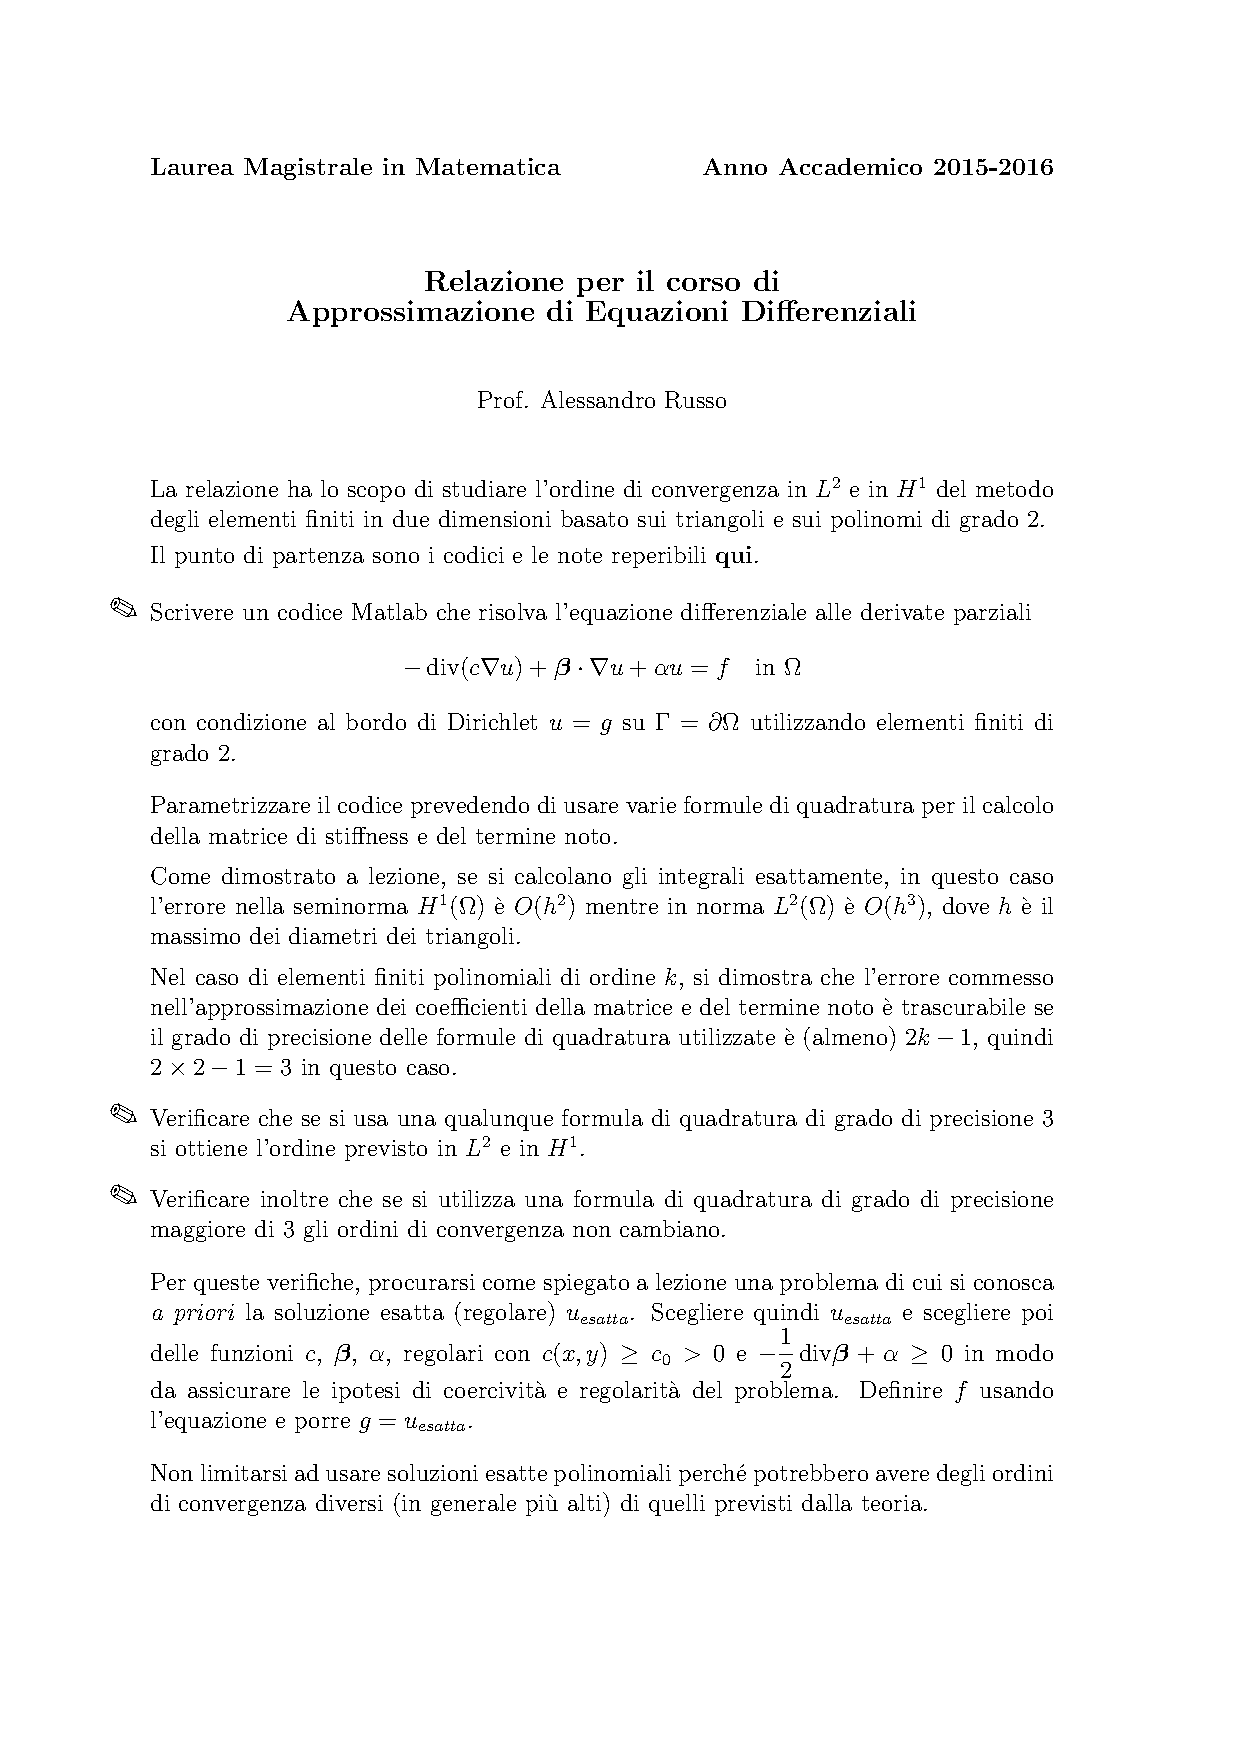
\includepdf[addtotoc={1,chapter,-,Testo Relazione,chap:project_test}, pages=-]{RelazioneProgettoEsame.pdf} 

\chapter{Elementi Finiti Per Problemi Ellittici}

\section{Introduzione}
In questo capitolo richiamiamo i concetti base del metodo agli elementi finiti per risolvere problemi ellittici del secondo ordine.\\
Il problema differenziale generale che affronteremo è del tipo:\\\\ \index{Problema Di Dirichlet} \label{Problema Di Dirichlet}
\begin{math}
\begin{system}
-div(c\nabla{u})+\beta \cdot \nabla{u} + \alpha u = f \qquad \qquad \ \Omega \\
u = g \qquad \qquad \qquad \qquad \qquad \qquad \qquad \quad \partial \Omega \\
\end{system}
\end{math}
\hfill \\\\
dove $\Omega \in \Re^{n}$ e dove con $\partial \Omega$ intendiamo il bordo relativo al dominio $\Omega$. I vari termini dell'equazione possono essere caratterizzati nel modo seguente:
\begin{itemize}
	\item \textbf{Termine Di Diffusione} $-div(c\nabla{u})$
	\item \textbf{Termine Di Avezione} $\beta \cdot \nabla{u}$
	\item \textbf{Termine Di Reazione} $\alpha u$	
\end{itemize}
Al bordo abbiamo considerato la condizione non omogenea di Dirichlet $u = g$. Sono possibili altri tipi di condizioni al bordo, ad esempio:
\begin{itemize}
	\item \textbf{Neumann} Condizione sulla derivata normale al bordo della funzione.
	\item \textbf{Cauchy} Impone al bordo sia una condizione di Dirichlet che una di Neumann.
	\item \textbf{Robin} Impone al bordo una condizione ottenuta come combinazione lineare di una condizione di Dirichlet e di una di Neumann.
\end{itemize}
L'equazione ellittica del secondo ordine è molto importante per la modellizzazione di problemi stazionari (ovveero indipendenti dal tempo), e infatti molte altre equazioni si riducono ad una riconducibile al caso ellittico nel regime stazionario \footnote{Ad esempio le equazioni di tipo parabolico e iperbolico sono equazioni ellittiche nelle variabili spaziali con l'aggiunta di termini temporali}. Forniamo alcuni esempi fisici modellizzati da questa equazione:
\begin{example} [Equazione di Poisson]
\hfill \\
Il caso più semplice è l'equazione di Poisson:\\\\
\begin{math}
\begin{system}
- \Delta u = f \qquad \qquad \quad \ \Omega \\
u = g \qquad \qquad \qquad \quad \partial \Omega \\
\end{system}
\end{math}
\hfill \\\\
dove $\Delta$ è l'operatore di Laplace, definito come:
\[ \Delta = div \nabla \]
Questa equazione modellizza ad esempio problema del calore stazionario \cite[Capitolo~3]{Salsa} o il problema generale dell'elettrostatica in presenza di cariche \cite[Capitoli~1,2,3]{Jackson}.
\qed
\end{example}
\begin{example} [Equazione di Fick Stazionaria]
\hfill \\
L'equazione di Fick descrive la variazione di concentrazione nei materiali in cui è presente diffusività molecolare ma non termica. Nel caso stazionario (ovvero che studia solo la diffusione spaziale senza considerare il tempo), abbiamo:\\\\
\begin{math}
\begin{system}
- D\Delta u + v \nabla u = f \qquad \qquad \quad \ \Omega \\
\partial_{\eta} u = 0 \quad \qquad \qquad \qquad \qquad \quad \partial \Omega \\
\end{system}
\end{math}
\hfill \\\\
dove al bordo sono state supposte condizioni di Neumann omogenee, a significare che non c'è diffusione attraverso il bordo del dominio (caso che invece avviene se ad esempio il bordo è poroso).
\qed
\end{example}
\hfill \\
Gli esempi qui posti sono tutti riguardanti quantità incognite scalari, che è il caso che considereremo in seguito. Il ragionamento può essere esteso a sistemi di equazioni ellittiche (ovvero a grandezze vettoriali). Ad esempio \cite[Capitolo~11]{BS} mostra un'applicazione delle tecniche qui presentate al problema bidimensionale dell'elasticità planare.

\section{Metodi Variazionali}
Vogliamo dunque risolvere un problema del tipo \ref{Problema Di Dirichlet}. Esso in particolare per essere ben definito richiedere ad esempio che la soluzione $u$ sia almeno di classe $C^2(\Omega)$. Questo limita molto la capacità di modellizzazione per problemi fisici reali (ad esempio che presentano discontinuità). Inolte non è detto che sia possibile trovare una soluzione in forma chiusa del problema. Per provare ad ovviare a questi problemi proviamo a passare ad una formulazione equivalente detta formulazione variazionale o debole, che permette alla funzione $u$ di essere meno regolare di quanto previsto dal problema differenziale. I riferimenti principali per questa sezione sono \cite{Brezis} e \cite{Evans}.\\
Consideriamo inizialmente il seguente problema omogeneo:\\\\
\index{Problema Di Dirichlet Omogeneo} \label{Problema Di Dirichlet Omogeneo}
\begin{math}
\begin{system}
-div(c\nabla{u})+\beta \cdot \nabla{u} + \alpha u = f \qquad \qquad \quad \ \Omega \\
u = 0 \quad \qquad \qquad \qquad \qquad \qquad \qquad \qquad \quad \partial \Omega \\
\end{system}
\end{math}
\hfill \\\\
ricordiamo inanzitutto la definizione di derivata debole:
\begin{definition} [\textbf{Derivata Debole}]  \index{Derivata Debole} \label{Derivata Debole}
\hfill \\
Per la formula di integrazione per parti abbiamo che se $f \in C^{\mid \alpha \mid}(\Omega)$ e $g \in C_{0}^{\mid \alpha \mid}(\Omega)$, con $\alpha$ multi-indice, allora vale:
\[ \int_{\Omega} { (\partial^{\alpha} f) \, g \; dx } \quad = \quad (-1)^{\mid \alpha \mid} \int_{\Omega} { f \, (\partial^{\alpha} \, g) \;dx } \]
da cui, se $f$ è localmente integrabile su $\Omega$, allora diciamo che una funzione $g$ è la sua $\alpha$-derivata debole, definita (quasi ovunque) come
\[ g = D^{ \alpha }f \]
se $\forall \phi \in  C_{0}^{\mid \alpha \mid}(\Omega)$ abbiamo
\[ \int_{\Omega} { g \, \phi \; dx } \quad = \quad (-1)^{\mid \alpha \mid} \int_{\Omega} { f \, (\partial^{\alpha} \phi) \; dx} \]
\qed
\end{definition}
\hfill \\
il concetto di derivata debole risulta quindi un'estensione a quello di derivazione classica, infatti ogni funzione di classe $C^k$ ha $k$-derivata debole.
Attraverso la definizione di derivata debole possiamo definire lo spazio di Sobolev $\mathbb{H}^{1}(\Omega)$:
\begin{definition} [\textbf{$\mathbb{H}^{1}(\Omega)$}] \index{Spazio $\mathbb{H}^{1}$} \label{Spazio H1}
\hfill \\
\[ \mathbb{H}^{1}(\Omega) \quad = \quad \left \{ v \in \mathbb{L}^{2}(\Omega): \quad \nabla{v} \in \mathbb{L}^{2}(\Omega) \right \}	\]
dove il gradiente è inteso come derivazione debole analogamente a come definito sopra. Questo spazio risulta essere uno spazio di Hilbert con prodotto scalare:
\[ < v, v' >_{\mathbb{H}^{1}(\Omega)} \quad = \quad < v, v' >_{\mathbb{L}^{2}(\Omega)} + < \nabla{v}, \nabla{v}' >_{\mathbb{L}^{1}(\Omega)}\]
ovvero con norma indotta dal prodotto scalare:
\[ \mid \mid v \mid \mid _{\mathbb{H}^{1}(\Omega)}\quad = \quad \mid \mid v \mid \mid _{\mathbb{L}^{2}(\Omega)} + \mid \mid \nabla{v} \mid \mid _{\mathbb{L}^{2}(\Omega)} \]
\qed
\end{definition}
Questo spazio è dunque l'insieme delle funzioni di $L^{2}(\Omega)$ con derivate deboli prime (espresse tramite il gradiente) anch'esse in $L^{2}(\Omega)$. In questo spazio (o in un suo sottospazio) andremo a cercare le soluzioni deboli della formulazione variazionale. \\
L'idea dietro alla formulazione debole è che il problema differenziale è scritto localmente. Vogliamo però scriverlo in forma globale, in modo da poter considerare funzioni meno regolari, attraverso il concetto di derivata debole.\\
\begin{theorem} [Problema Ellitico In Forma Variazionale] \index{Problema Ellittico Debole} \label{Problema Ellittico Debole}
\hfill \\
Il problema ellittico \ref{Problema Di Dirichlet Omogeneo} può essere riscritto in forma variazionale nel seguente modo:\\
Trovare $u \in  \mathbb{V} \, = \, \mathbb{H}^{1}(\Omega)$ tale che:
\[ \int_{\Omega}{c \, \nabla u \nabla v \; dx} \; + \; \int_{\Omega}{(\beta \cdot \nabla u) \, v \; dx} \; + \; \int_{\Omega}{\alpha \, u \, v \; dx} \quad = \quad \int_{\Omega}{f \, v \; dx} \qquad \forall v \in \mathbb{V} \, = \, \mathbb{H}^{1}(\Omega) \]
dove $u$ è detta soluzione debole del problema variazionale.
\end{theorem}
\hfill \\
\emph{Dimostrazione}\\
Condideriamo l'equazione
\[ -div(c\nabla{u}) \ + \ \beta \cdot \nabla{u} \ + \ \alpha u \ = \ f \]
e moltiplichiamo entrambi i membri per una funzione $v \in C^{\infty}(\Omega)$:
\[ -div(c\nabla{u}) \, v \ + \ (\beta \cdot \nabla{u}) \, v \ + \ \alpha u v \ = \ f \, v\]
integriamo dunque su tutto il dominio $\Omega$ rispetto alla misura di Lebesgue $dx$ del dominio:
\[ - \ \int_{\Omega}{div(c\nabla{u}) \, v \; dx} \ + \ \int_{\Omega}{(\beta \cdot \nabla{u}) \, v \; dx} \ + \ \int_{\Omega}{\alpha \, u \, v \; dx} \ = \ \int_{\Omega}{f  \, v \; dx}\]
consideriamo il primo integrale. Per le proprietà della divergenza se $f$ è una funzione scalare e se $\mathbb{F}$ è un campo vettoriale, allora vale:
\[ div(f \mathbb{F}) \ = \  \nabla f \cdot \mathbb{F} \ + \ f div(\mathbb{F})\]
considerando dunque $f \ = \ v$ e $\mathbb{F} \ = c \nabla u$, abbiamo
\[ div(v c \nabla u) \ = \  \nabla v (c \nabla u) \ + \ v \, div(c \nabla u)\]
ovvero
\[ v \, div(c \nabla u) \ = \ div(v \, c \, \nabla u) \ - \ c \, \nabla v \nabla u \]
sostituendo nell'integrale abbiamo
\[ - \ \int_{\Omega}{div(c\nabla{u}) \, v \; dx} \ = \ \int_{\Omega}{c \, \nabla v \nabla u \; dx} \ - \ \int_{\Omega}{div(v \, c \nabla u) \; dx}\]
possiamo quindi applicare il teorema della divergenza
\[ \int_{\Omega}{div(v \, c \nabla u) \; dx} \ = \ \int_{\partial \Omega}{ (v \, c \nabla u) \cdot \eta \, \, \; d \sigma (x)}\]
dove $\eta$ è il versore normale e $d \sigma (x) $ è la misura superficiale dell'ipersuperficie $(n-1)$-dimensionale $\partial \Omega $ \footnote{La misura superficiale differisce dalla misura di Lebesgue in quanto tiene conto anche della curvatura dello spazio}. La funzione $u$ è però nulla sul bordo, e quindi l'integrale su $\partial \Omega$ è nullo. Otteniamo cosi la forma debole:
\[ \int_{\Omega}{c \, \nabla u \nabla v \; dx} \; + \; \int_{\Omega}{(\beta \cdot \nabla u) \, v \; dx} \; + \; \int_{\Omega}{\alpha \, u \, v \; dx} \quad = \quad \int_{\Omega}{f \, v \; dx} \]
dobbiamo però caratterizzare la regolarità delle funzioni $u$, $v$ e $f$ presenti, affinche questa forma debole sia ben definita.
Inanzitutto sia $u$ che $v$ devono avere derivata debole di ordine $1$. Affinchè poi gli integrali siano definiti e convergenti, dobbiamo avere che $u$, $v$, ed $f$ devono essere almeno in $L^{2}(\Omega)$, cosi come i gradienti (intesi nel senso della derivazione debole) di $u$ e $v$. Ciò implica quindi che sia $u$ che $v$ devono appartenere a $ \mathbb{V} \, = \, \mathbb{H^1}(\Omega)$. Inoltre abbiamo imposto le condizioni omogeneee di Dirichlet. Possiamo quindi considerare il sottospazio di funzioni di $ \mathbb{V} \, = \, \mathbb{V}_{0} \, = \,\mathbb{H}_{0}^{1}(\Omega)$: \index{Spazio $\mathbb{H}_{0}^{1}$} \label{Spazio H01}
\[  \mathbb{V}_{0} \, = \, \mathbb{H}_{0}^{1}(\Omega) \ = \ \left \{ \, v \in \mathbb{H}^{1}(\Omega) \, :  \, \restr{v}{\partial \Omega} = 0 \, \right \} \ \subset \  \mathbb{H}^1(\Omega) \]
da cui risulta che
\begin{itemize}
	\item $f \in L^{2}(\Omega)$
	\item $u, \, v \in \mathbb{H}_{0}^{1}(\Omega) \ \subset \mathbb{H}^{1}(\Omega)$
\end{itemize}
\qed
\hfill \\
allo stesso modo si può procedere per il caso non omogeneo \ref{Problema Di Dirichlet}, dove però al bordo l'integrale non è più nullo, ma va considerato con $u = g$ a livello di tracce.
\hfill \\
Il problema in forma debole \ref{Problema Ellittico Debole}, può essere espresso in forma astratta:
\begin{definition} [Problema Astratto] \index{Problema Astratto} \label{Problema Astratto}
\hfill \\
Trovare $u \in  \mathbb{V}$, con $\mathbb{V}$ spazio di Hilbert, tale che
\[ a(u,v) = F(v) \qquad \qquad \forall v \, \in \mathbb{V} \]
dove
\begin{itemize}
	\item $a: V \times V \rightarrow \Re \quad $ è una forma bilineare 
	\item $F: V \rightarrow \Re \quad $ è un funzionale lineare, ovvero $F \in \mathbb{V}'$.
\end{itemize}
\qed
\end{definition}
Nel nostro caso particolare \ref{Problema Ellittico Debole}  il problema astratto è formato da:
\begin{definition} [Problema ellittico astratto] \index{Problema Ellittico Astratto} \label{Problema Ellittico Astratto}
\hfill \\
\begin{itemize}
	\item $\mathbb{V} = \mathbb{H}^1(\Omega)$
	\item $a(u,v) \ = \ \int_{\Omega}{c \, \nabla u \nabla v \; dx} \; + \; \int_{\Omega}{(\beta \cdot \nabla u) \, v \; dx} \; + \; \int_{\Omega}{\alpha \, u \, v \; dx}$
	\item $F(v) \ = \ \int_{\Omega}{f \, v \; dx}$
\end{itemize}
\qed
\end{definition}
Il lemma di Lax-Milgram fornisce un risultato di esistenza e unicità della soluzione (debole) al problema astratto, che coincide dunque con l'esistenza e unicità della soluzione di \ref{Problema Ellittico Debole} e di \ref{Problema Di Dirichlet}:
\begin{theorem} [Lax-Milgram - 1954] \index{Lemma di Lax-Milgram} \label{Lemma di Lax-Milgram}
\hfill \\
Esiste ed è unica la soluzione debole $u \in \mathbb{V}$ di Hilbert per il problema astratto \ref{Problema Astratto} se:
\begin{itemize}
	\item $a(u,v)$ è continua: $\qquad a(u,v) \ \leq \ M \mid \mid u \mid \mid_{\mathbb{V}} \, \mid \mid v \mid \mid_{\mathbb{V}}$
	\item $a(u,v)$ è coerciva: $\qquad \ a(v,v) \ \geq \ c \mid \mid v \mid  \mid_{\mathbb{V}}^{2}$
	\item $F(v)$ è continua: $\qquad \quad F(v) \ \leq \ C \mid \mid v \mid \mid_{\mathbb{V}}$
\end{itemize}

\end{theorem}
Questo lemma è stato in seguito generalizzato da Babuska \cite{babuska1971BLM}, in modo da considerare due spazi di appartenzenza diversi per $u$ e per $v$ e indebolendo la richiesta sulla coercività (richiedendo la coercività debole).\\
Nel caso in cui $a(u,v)$ sia anche simmetrica, tale forma è un prodotto scalare, e il lemma di Lax-Milgram deriva direttamente dal teorema di rappresentazione di Riesz. \\
Nel caso particolare di \ref{Problema Ellittico Astratto}, si può dimostrare che affinchè valgano le condizioni delle ipotesi del lemma di Lax-Milgram \ref{Lemma di Lax-Milgram}, le funzioni caratterizzanti il problema devono rispettare le seguenti:
\begin{itemize}
	\item $c(\underline{x}) \in L^{\infty} \qquad c_{max} \ \geq \ c(\underline{x}) \ \geq \ c_{min} \ > \ 0 $
	\item $\alpha(\underline{x}) \in L^{2}(\Omega), \ \beta(\underline{x}) \in C^{1}(\Omega) \qquad \alpha \, - \, div \beta \ = \ 0$
	\item $f(\underline{x}) \in L^{2}(\Omega)$
\end{itemize}
{ \color{red} MIGLIORARE DESCRIZIONE CASO NON OMOGENE0\\}
{ \color{blue} FINE SEZIONE\\}

\section{Metodo Galerkin}
Abbiamo visto che il problema astratto \ref{Problema Ellittico Astratto} ammette soluzione unica se la forma bilineare $a(u,v)$ è continua e coerciva, e se la forma lineare $F(v)$ è continua per il lemma di Lax-Milgram \ref{Lemma di Lax-Milgram}. Non esiste però un metodo generale per trovare la soluzione esatta al problema astratto in forma chiusa su un qualunque dominio $\Omega$ (soluzione che non è detto che sia formulabile in forma chiusa). Per risolvere il problema dobbiamo quindi tentare di stimare la soluzione esatta con una soluzione approssimata, valutandone poi l'errore di approssimazione. La principale bibliografia per questa sezione è formata da \cite{BS} e da \cite{Ciarlet} e \cite{Q}.\\
Uno dei metodi principali che consente questo processo è quello di Galerkin \footnote{Un altro metodo rilevante, ma più semplice è quello delle differenze finite, in cui si approssimano direttamente le derivate sui nodi per riformulare l'equazione in modo approssimato}:
\begin{definition} [Metodo Galerkin] \index{Metodo Galerkin} \label{Metodo Galerkin}
\hfill \\
Il metoodo Galerkin consiste nell'approssimare lo spazio continuo $\mathbb{V}$ con una famiglia di spazi $\mathbb{V}_{h}$, dipendenti da un parametro positivo $h$, tali che:
\begin{itemize}
	\item $\mathbb{V}_{h} \subset \mathbb{V}$
	\item $dim \left( \mathbb{V}_{h} \right) \ = \ N_{h} \ \ < \ \ \infty \qquad \forall h > 0 \qquad \qquad ( \text{Ovvero ogni} \ \mathbb{V}_{h} \ \text{è uno spazio discreto} )$
\end{itemize}
In questo modo possiamo riscrivere il problema astratto in forma discreta sul singolo spazio $\mathbb{V}_{h}$:
\center{\emph{Trovare $u_{h} \in  \mathbb{V}_{h}$, tale che} $ a(u_{h},v_{h}) = F(v_{h}) \qquad \qquad \forall v_{h} \, \in \mathbb{V}_{h} $}\\
\hfill \\
detta equazione di Galerkin. \footnote{Notiamo che la forma dell'equazione non cambia tra il problema continuo e quello discreto, cambiano invece gli spazi con cui lavoriamo}
\qed
\end{definition}
\hfill \\
dato che $\mathbb{V}_{h} \subset \mathbb{V}$, continuano a valere le ipotesi del lemma di Lax-Milgram \ref{Lemma di Lax-Milgram}, e quindi la soluzione al problema discreto esiste ed è unica. Inoltre vale la seguente relazione tra la soluzione del problema continuo e quella del problema approssimato:
\begin{definition} [Ortogonalità Di Galerkin] \index{Ortogonalità di Galerkin} \label{Galerkin Orthogonality}
\hfill \\
Sia $u$ la soluzione esatta del problema continuo e sia $u_{h}$ la soluzione del problema discreto. Definito l'errore $\epsilon_{h}$ come
\[ \epsilon_{h} \ = \ u \, - \, u_{h} \]
allora abbiamo che, sottraendo i due problemi membro a membro
\[ a(u,v) \, - \, a(u_{h}, v_{h}) \ =  \ f(v) \, - \, f(v_{h}) \]
possiamo perè restringere le funzioni $v$ allo spazio $\mathbb{V}_h$, ovvero considerare
\[ a(u,v_{h}) \, - \, a(u_{h}, v_{h}) = f(v_{h}) \, - \, f(v_{h}) = 0) \]
per linearità della forma $a$ abbiamo
\[ a(u,v_{h}) \, - \, a(u_{h}, v_{h}) \ =  \ a(u \, - \, u_{h}, v_{h}) \ =  \ a(\epsilon_{h},v_{h}) = 0 \]
nel caso in cui la forma $a(\cdot,\cdot)$ sia simmetrica (ovvero è un prodotto scalare), abbiamo che l'errore $\epsilon_{h}$ è ortogonale ad ogni funzione $\forall v_{h} \in \mathbb{V}_{h}$, e quindi è ortogonale all'intero spazio $\mathbb{V}_{h}$.
\qed
\end{definition}
\hfill \\
E' possibile inoltre dare una stima dell'errore compiuto, attraverso il lemma di Cèa:
\begin{theorem} [Lemma di Cèa] \index{Lemma Di Cèa} \label{Lemma Di Cea}
\hfill \\
L'errore compiuto con l'approssimazione tramite il problema discreto permette la seguente stima:
\[ \mid \mid \ u \, - \, u_{h} \ \mid \mid_{\mathbb{V}(\Omega)} \quad \leq \quad \frac{M}{c} \ Inf_{v_{h} \in \mathbb{V}_{h}} \mid \mid \ u \, - \, v_{h} \ \mid \mid_{\mathbb{V}(\Omega)} \]
dove $M$ è la costante della continuità e $c$ quella della coercività di $a(\cdot,\cdot)$.
\qed
\end{theorem}
\hfill \\
L'approssimazione tramite lo spazio $\mathbb{V}_{h}$ consente inoltre di trasformare il problema continuo in un sistema lineare di equazioni. Dato che lo spazio $\mathbb{V}_{h}$ è un sottospazio vettoriale finito, possiamo considerarne una base
\[ \overline{\phi} = \left \{ \phi_{i} \right \} \qquad \qquad i = 1,..., n = \dim{V_{h}} \]
e quindi possiamo sviluppare la funzione $u_{h}$ rispetto ad essa:
\[ u_{h} = \sum_{i = j}^{n} u_{j} \ \phi_{j} \]
è inoltre possibile dimostrare che l'approssimazione vale anche considerando il problema solo riferito alle basi\footnote{Questo in quanto possiamo scrivere ogni funzione $v_{h}$ dello spazio $\mathbb{V}_{h}$ come combinazione lineare delle basi}, ovvero sostituendo alle funzioni $v_{h}$ le funzioni di base $\phi_{i}$
\[ a \ \left( \sum_{j = 1}^{n} u_{j} \ \phi_{j} \ , \ \phi_{i} \right) \ = \ F \ \left(  \phi_{i} \right) \]
Sfruttando la linearità di $a(\cdot,\cdot)$ otteniamo:
\[ \sum_{j = 1}^{n} u_{j} \ a \, \left( \phi_{j} \ , \ \phi_{i} \right) \ = \ F \ \left(  \phi_{i} \right) \]
e sommando su tutte le funzioni di base (ovvero rispetto all'indice $i$):
\[ \sum_{i = 1}^{n} \sum_{j = 1}^{n} u_{j} \ a \, \left( \phi_{j} \ , \ \phi_{i} \right) \ = \ \sum_{i = 1} F \ \left(  \phi_{i} \right) \]
ovvero abbiamo ridotto il problema ad un sistema lineare di equazioni, definendo dunque il problema astratto discreto in forma matriciale:
\begin{definition} [Problema Astratto Discreto In Forma Matriciale] \index{Problema Astratto Discreto In Forma Matriciale} \label{Problema Astratto Discreto In Forma Matriciale}
\hfill \\
Trovare $\underline{u}  \in \Re^{n}$ tale che
\[ K_{h} \, \underline{u} \; = \; \underline{f} \]
dove abbiamo definito la matrice di stiffness $Kh$ \index{Matrice Di Stiffness} \label{Matrice Di Stiffness} e il vettore termine noto $\underline{f}$ come:
\[ (K_{h})_{i,j} \ = \ a \, \left( \phi_{j} \ , \ \phi_{i} \right) \qquad \qquad \qquad (\underline{f})_{i} \ = \ F \ \left(  \phi_{i} \right) \]
\qed
\end{definition}
\hfill \\
Nel caso particolare del problema ellittico astratto \ref{Problema Ellittico Astratto} abbiamo la matrice di stiffness \index{Matrice Di Stiffness Problema Ellittico} \label{Matrice Di Stiffness Problema Ellittico}
\[ (K_{h})_{i,j} \ = \ a(u,v) \ = \ \int_{\Omega}{c \, \nabla \phi_{j} \nabla \phi_{i} \; dx} \; + \; \int_{\Omega}{(\beta \cdot \nabla \phi_{j}) \, \phi_{i} \; dx} \; + \; \int_{\Omega}{\alpha \, \phi_{j} \, \phi_{i} \; dx} \]
e il vettore termine noto:
\[ (\underline{f})_{i} \ = \ F \ \left(  \phi_{i} \right) \ = \ \int_{\Omega}{f \, \phi_{i} \; dx} \]
{ \color{red} CONTROLLARE LA CORRETTEZZA DEGLI INDICI RISPETTO A QUANTO FATTO A LEZIONE\\}
{ \color{blue} FINE SEZIONE\\}


\section{Approssimazione Con Elementi Finiti}
Il metodo di Galerkin fornisce l'idea di approssimare il problema continuo con quello discreto, ma non da vincoli su come fare questa approssimazione. Gli elementi finiti sono un metoodo di Galerkin in cui l'approssimazione viene fatta considerando polinomi su elementi di una partizione (poligonale) del dominio. I testi di riferimento sono \cite{BS} e da \cite{Ciarlet} e \cite{Q}. In particolare lavoriamo in questa sezione considerando per semplicità un dominio $\Omega \in \Re^{2}$, con l'ovvia estensione al caso in più di due dimensioni.
Il fondamento del metodo agli elementi finiti è di costruire lo spazio discreto $\mathbb{V}_h$ tramite funzioni polinomiali da considerare sugli elementi di una mesh rappresentante $\Omega$. \\
L'idea di costruire una mesh per il dominio $\Omega$ si basa sul concetto topologico di complesso simpliciale euclideo \cite[Chapter~2]{FerrarioSimpl}, che nel caso particolare  bidimensionale permette di considerare la scomposizione di un dominio poligonale in un numero finito di triangoli (e quindi fare una triangolazione del dominio) seguendo le due seguenti proprietà:
\begin{itemize}
	\item Un vertice di un triangolo $\mathbb{T}_{i}$ può essere un punto di un qualsiasi altro triangolo $\mathbb{T}_{j}$ solo se è un vertice dell'altro triangolo. Questo impedisce che un triangolo abbia un verice nel lato di un'altro (ovvero impone la conformità dei triangoli).
	\item Se l'intersezione degli interni di due triangoli non è vuota, allora i due triangoli devono coincidere. Questa proprietà serve ad escludere triangoli uno interno all'altro o incastonati.
\end{itemize}
Nel seguito del paragrafo ci riferiremo per semplicità a domini poligonali, in particolare al quadrato di lato unitario con un vertice nell'origine e con due lati sugli assi$x$ e $y$. Nel caso più generale in cui il dominio non sia poligonale, bisognerà trovare delle tecniche di approssimazione per poter comunque generare una sua triangolazione e quindi crearne una mesh.\footnote{Questo si basa sull'idea di varietà triangolabile, ovvero omeomorfa ad un poliedro \cite[Chapter~5]{FerrarioSimpl}. A livello pratico ciò può essere fatto ad esempio con il metodo isoparametrico \cite{lenoir1986optimal} o con l'analisi isogeometrica che si interfaccia alla progettazione CAD \cite{CHYisogeometric}}. Definiamo dunque un elemento finito:
\begin{definition}[Elemento Finito] \index{Elemento Finito} \label{Elemento Finito}
\hfill \\
Definiamo un elemento finito come una terna $( \mathbb{T} \, , \, \mathbb{P} \, , \, \Sigma )$, dove:
\begin{itemize}
	\item $\mathbb{T}$ è l'insieme dei triangoli della mesh sul dominio $\Omega$, ovvero è il complesso simpliciale associato\footnote{Non è unico, ma allo stesso dominio $\Omega$ possiamo associare più complessi simpliciali} al dominio $\Omega$.
	\item $\mathbb{P}$ è lo spazio locale che utilizziamo per l'approssimazione.
	\item $\Sigma$ è l'insieme dei gradi di libertà $\quad \Sigma = \left \{ \Sigma_{i} : \mathbb{P} \rightarrow \Re \quad \text{lineare} \right \}_{i=1}^{dim \mathbb{P}} $
\end{itemize}
\qed
\end{definition}
\hfill \\
Attraverso gli elementi finiti possiamo costruire lo spazio $\mathbb{V}_{h}$ come il sottoinsieme di $\mathbb{V}$ tale che i suoi elementi siano localmente (ovvero su ogni triangolo) esprimibili come elementi dello spazio $\mathbb{P}$ e soddisfacenti alcune condizioni ulteriori per garantire la regolarità del problema discreto cosi formulato. In particolare considereremo in seguito elementi cosi definiti:
\begin{definition}[Elementi Finiti Polinomiali] \index{Elementi Finiti Polinomiali} \label{Elementi Finiti Polinomiali}
\hfill \\
Considereremo come spazio locale di approssimazione $\mathbb{P} = \mathbb{P}_{k}(T)$, ovvero lo spazio dei polinomi di grado $k$ sull'elemento $T$, mentre definiamo lo spazio $\mathbb{V}_{h}$ come:
\[ \mathbb{V}_{h} \ = \ \left \{ \, v \in \mathbb{H}_{g}^{1}(\Omega) \, :  \, \restr{v}{\partial \Omega} = g \, , \, \restr{v}{T} \in  \mathbb{P}_{k}(T) \ \ \forall T \in \mathbb{T} \ \right \} \ \subset \  \mathbb{H}_{g}^{1}(\Omega) \ = \ \mathbb{V} \]
Avremo poi in generale un numero $N$ gradi di libertà, definito come
\[ N \ = \ dim \left( \mathbb{P}_{k}(\Omega) \right) \ = \ \binom{n+k}{k} \ = \ \frac{(n+k)!}{k! \cdot (n!)} \]
dove $n$ è la dimensione dello spazio $\Omega$. Nel nostro caso particolare $n \, = \, 2$, e quindi sui triangoli avremo per i polinomi di grado $k$ un numero di gradi di libertà pari a:
\[ N \ = \ dim \left( \mathbb{P}_{k}(T) \right) \ = \ \binom{2+k}{k} \ = \ \frac{(2+k)!}{k! \cdot (2!)} \ = \ \frac{(2+k) \cdot (1+k) \cdot k!}{2 \cdot k!} \ = \ \frac{(k+2) \cdot (k+1)}{2} \]
\qed
\end{definition}
\hfill \\
Per ricondurci alla definizione data del metodo di Galerkin \ref{Metodo Galerkin}, si considera una famiglia di spazi $\mathbb{V}_{h}$ analoghi alla definizione appena data e dipendenti dal parametro positivo $h$ che rappresenta il diametro massimo dei triangoli della mesh. In particolare il  metodo agli elementi finiti in versione $h$ consiste nel far tendere questo diametro a zero per riottenere il problema continuo. Quello che si fa nella pratica è un'analisi a posteriori dell'errore, nella quale si fissa una certa tolleranza sull'errore compiuto e si usa una versione adattiva del metodo, ovvero si varia automaticamente il parametro $h$ (e quindi si raffina la partizione) per ottenere una soluzione approssimata con la precisione richiesta. Altre varianti sono possibili, quali il metodo $p$ \cite{babuvska1981p}, in cui la triangolazione è fissata, ma si usano polinomi di grado $p$ crescente o il metodo $hp$ \cite{babuvska1994hp} che usa una fusione tra i metodi due metodi $h$ e $p$.\\
\hfill \\
Definiamo ora una base per questo spazio $\mathbb{V}_{h}$ come definito in \ref{Elementi Finiti Polinomiali}, in modo da poter esplicitare il problema ellittico debole in forma matriciale \ref{Matrice Di Stiffness Problema Ellittico}:
\begin{definition} [Base di Lagrange] \index{Base di Lagrange} \label{Base di Lagrange}
\hfill \\
Definiamo la base di Lagrange $\phi_{i}$ per lo spazio $\mathbb{V}_{h}$ in corrispondenza del nodo libero $v_{j}$ come alla funzione:
\begin{center}
\begin{math}
\phi_{i}(v_{j}) = \left\{ \begin{array}{ll}
         1 \qquad & \mbox{if $\ i \, = \, j$}\\
         0 \qquad & \mbox{if $\ i \, \neq \, j$}\end{array} \right.
\end{math}
\end{center}
In particolare notiamo che il supporto della funzione $\phi_{i}$ è formata dai triangoli che circondano il vertice $v_{i}$.
\qed
\end{definition}
\hfill \\
Usando questa base, la risultante matrice di stiffness $K_{h}$ oltre ad essere definita positiva \footnote{Fatto che vale per ogni base}, risulta essere anche una matrice sparsa \footnote{Che invece vale in particolare per questa base ma non in generale}. Ciò permette da un lato di ridurre le dimensioni in memoria della matrice e dall'altro di usare metodi appositi per la risoluzione di sistemi lineari con matrice associata sparsa, quali il gradiente coniugato o l'uso di precondizionatori \cite{SaadSparse}.\\
Definiamo dunque il problema astratto discreto agli elemeti finiti come al caso particolare del problema astratto discreto in forma matriciale \ref{Problema Astratto Discreto In Forma Matriciale} dove consideriamo come basi le basi di Lagrange \ref{Base di Lagrange} e gli spazi cosi come definiti nel caso degli elementi finiti polinomiali \ref{Elementi Finiti Polinomiali}. In modo analogo definiamo il problema agli elementi finiti che approssima il problema ellittico in forma debole \ref{Problema Ellittico Debole}.

\chapter{Calcolo Esplicito}
In questo capitolo mostriamo come fare esplicitamente il calcolo della soluzione approssimata tramite gli elementi finiti. Quello che andiamo a risolvere è dunque il problema \ref{Problema Astratto Discreto In Forma Matriciale} rappresentato dal seguente sistema lineare
\[ K_{h} \, \underline{u} \; = \; \underline{f} \]
che scritto esplicitamente rispetto alla definizione del problema ellittico in forma astratta \ref{Problema Ellittico Astratto} porta a dover calcolare
\[\int_{\Omega}{c \, \nabla \phi_{j} \nabla \phi_{i} \; dx} \; + \; \int_{\Omega}{(\beta \cdot \nabla \phi_{j}) \, \phi_{i} \; dx} \; + \; \int_{\Omega}{\alpha \, \phi_{j} \, \phi_{i} \; dx} \quad = \quad \int_{\Omega}{f \, \phi_{i} \; dx}\]
dove $\underline{\phi}$ è la base di Lagrange \ref{Base di Lagrange} mentre $c, \beta, \alpha$ e $f$ sono i dati del problema.\\
Dato che la base di Lagrange ${\phi}_{i}$ ha supporto compatto formato dai vertici $j$ vicini al vertice $i$ (ovvero appartenenti ai triangoli adiacenti a quello in cui è contenuto $i$), possiamo limitarci a fare il calcolo su ogni singolo triangolo considerando che solo i termini con vertici $i$,$j$ appartenente al triangolo corrente risultano non zero, per poi sommare nella matrice $K_{h}$ tutti i contributi \footnote{Questo risultato è legato strettamente al fatto che la matrice $K_{h}$ sia sparsa}. Scomponiamo quindi la matrice di stiffness $K_{h}$ \ref{Matrice Di Stiffness Problema Ellittico} in una somma matrici elementari $K_{h}^{T}$ tali che:
\[ (K_{h})_{ij} \quad = \quad \sum_{T \in \mathbb{T}}{(K_{h}^T)_{ij}} \quad = \quad \sum_{T \in \mathbb{T}} \bigg(  \int_{T}{c \, \nabla \phi_{j} \nabla \phi_{i} \; dx} \; + \; \int_{T}{(\beta \cdot \nabla \phi_{j}) \, \phi_{i} \; dx} \; + \; \int_{T}{\alpha \, \phi_{j} \, \phi_{i} \; dx} \bigg)\]
Allo stesso modo facciamo per il termine noto:
\[ (f)_{i} \quad = \quad \sum_{T \in \mathbb{T}}{(f^T)_{i}} \quad = \quad \sum_{T \in \mathbb{T}} \int_{T}{f \, \phi_{i} \; dx}\]
Consideriamo dunque $\forall \ T \in \mathbb{T}$ il problema:
\[ \int_{T}{c \, \nabla \phi_{j} \nabla \phi_{i} \; dx} \; + \; \int_{T}{(\beta \cdot \nabla \phi_{j}) \, \phi_{i} \; dx} \; + \; \int_{T}{\alpha \, \phi_{j} \, \phi_{i} \; dx} \quad = \quad \int_{T}{f \, \phi_{i} \; dx}\]
Affrontiamo subito il problema delle condizioni al bordo. Nei vertici di bordo sappiamo già il valore della soluzione $u$, che corrisponde al valore del dato al bordo $g$ calcolato nel vertice.



Dato che il calcolo diretto viene abbastanza complicato in più di una dimensione, usiamo l'idea di ricondurci ad un elemento di riferimento.


\chapter{Stime Sugli Errori}

\section{Stime Teoriche Errori}
Raccogliamo in questa sezione varie stime per l'errore compiuto nell'approssimazione agli elementi finiti. Inanzitutto ricordiamo il lemma di Cea \ref{Lemma Di Cea} per la stima dell'errore compiuto dal metodo Galerkin \ref{Metodo Galerkin}:
\[ \mid \mid \ u \, - \, u_{h} \ \mid \mid_{\mathbb{V}(\Omega)} \quad \leq \quad \frac{M}{c} \ Inf_{v_{h} \in \mathbb{V}_{h}} \mid \mid \ u \, - \, v_{h} \ \mid \mid_{\mathbb{V}(\Omega)} \]
dove $M$ è la costante della continuità e $c$ quella della coercività di $a(\cdot,\cdot)$. Vogliamo però dare delle stime dell'errore compiuto dall'approssimazione agli elementi finiti in varie norme.

\section{Calcolo Errore $\mathbb{L}^{2}$}

\section{Calcolo Errore $\mathbb{H}^{1}$}



{ \color{red} DA AGGIUNGERE STIME ERRORI ELEMENTI FINITI\\}
{ \color{blue} FINE SEZIONE\\}

\chapter{Codice Matlab}
\lstdefinestyle{matlab}{
  belowcaptionskip=1\baselineskip,
  breaklines=true,
  frame=L,
  %xleftmargin=\parindent,
  %xleftmargin=\hangindent,
  language=matlab,
  showstringspaces=false,
  basicstyle=\footnotesize\ttfamily,
  keywordstyle=\bfseries\color{green!40!black},
  commentstyle=\itshape\color{purple!40!black},
  identifierstyle=\color{blue},
  stringstyle=\color{orange},
}

Riportiamo di seguito il codice Matlab in cui si presenta un'implementazione del metodo agli elementi finiti per il problema ellittico \ref{Problema Di Dirichlet} nel caso particolare di un dominio $\Omega \in \Re^{2}$. Riportiamo solo il programma principale \emph{fem2.m}, mentre le altre funzioni di supporto utilizzate (come ad esempio per la generazione della mesh, per le formule di quadratura o per i grafici), possono essere trovate online al sito \url{https://github.com/UniversityProjects/FEM1/tree/master/Project}
%\lstinputlisting[language=Matlab]{fem2.m}
\lstinputlisting[caption=Elementi Finiti Di Ordine Due Per Il Problema Ellittico, style=matlab]{fem2.m}


\chapter{Esperimenti Numerici}
Consideriamo in questo capitolo un confronto tra soluzione esatta e soluzione approssimata per verificare a livello pratico i risultati teorici di convergenza rispetto al parametro geometrico $h$ della specifica mesh.


\printindex

% \bibliographystyle{ieeetr}
\bibliographystyle{alpha}
%\bibliographystyle{plain}
\bibliography{mybib,pde_num}
\addcontentsline{toc}{chapter}{Bibliography}

\end{document}
